\chapter{SSOScan: Automatic Vulnerability Scanner}
\label{sec:ssoscan}

Chapter~\ref{sec:explication} demonstrates that service provider's documentation and SDKs are far from perfect and often missing implicit security-critical assumptions, and an exploratory study in Chapter~\ref{sec:explicating_test} shows that many application developers are prone to miss such assumptions which may cause serious vulnerabilities.  

To better understand and mitigate these risks, we present our design and implementation of SSOScan in this Chapter, an automated vulnerability checker for applications using SSO.  SSOScan carries out simulated attacks automatically by observing the application and monitors the application behavior through this process to determine vulnerability status.  Compared to the manual studies we presented in Chapter~\ref{sec:explicating_test}, SSOScan is capable of successfully checking 80\% of high-profile web applications in a short period of time per test without requiring any human interaction.  

SSOScan prototype focuses on Facebook as the identity provider, but our approach is generic and could be applied to check other identity providers as well.  It takes a website URL as input, determines if that site uses Facebook SSO, and automatically signs into the site using Facebook test accounts and completes the registration process when necessary.  Then, SSOScan simulates several attacks on the site while observing the responses and monitoring network traffic to automatically determine if the application is vulnerable to any of the tested vulnerabilities.  In addition to Single Sign-On services, many of the automation heuristics and techniques could also be adapted to scan for vulnerabilities in integrating other security-critical services such as online payments and file sharing APIs.

For the rest of this Chapter, we first show in Chapter~\ref{sec:ssoscan_manual_example} the human effort involved in manually checking an example application for the assumption IE vulnerability status mentioned in Chapter~\ref{sec:explicating_illustrative_example}.  This gives readers a general idea of what actions SSOScan needs to automate.  Then, we discuss some closely related works in this field in Chapter~\ref{sec:ssoscan_related_work}, and the vulnerabilities SSOScan aims to detect in Chapter~\ref{sec:ssoscan_vuls}.  In Chapter~\ref{sec:ssoscan_design} we explain the design and implementation of SSOScan, and present the large-scale study results we obtained by using SSOScan to check the top 20,000-ranked websites according to Quantcast in Chapter~\ref{sec:ssoscan_study}.  Our exploration experiments and results to improve SSOScan's speed and automation success rate are given in Chapter~\ref{sec:ssoscan_heuristics}.  Finally, we discuss the vendor responses we got and possible deployment scenarios for SSOScan in Chapter~\ref{sec:ssoscan_deployment}.

\section{A Manual Scanning Example}
\label{sec:ssoscan_manual_example}

For reader's convenience, we recap the vulnerability previously mentioned in Chapter~\ref{sec:explicating_illustrative_example}.  The vulnerability exists because the application uses \emph{access\_token} as the only credential to authenticate users through Facebook SSO, and \emph{access\_token} is not tied to a particular application.  Denoting Mallory as the malicious party, Alice as the victim, and Foo as the vulnerable application, this vulnerability can be exploited using the following steps:  (0.0) Alice and Mallory both own accounts at IdP.  (0.1) Mallory lures Alice to use Mallory's rogue application, through which Mallory obtains Alice's \emph{access\_token} for the rogue application as a preparation stage for the attack.  (0.2) We assume Alice uses Foo application previous to the attack.  (1) Mallory performs necessary actions to log in to Foo using Mallory's own IdP account.  (2) As the IdP returns the \emph{access\_token} to Mallory's browser, Mallory swaps it with the previously obtained \emph{access\_token} from Alice.  (3) 
Mallory checks with the browser to see if Foo has indeed authenticated Mallory as Alice, i.e. if Foo is vulnerable to this impersonation attack.

Playing as both the victim and the perpetrator, these steps are essentially what we did to test the 27 applications in Chapter~\ref{sec:explicating_test}, and here we list the actual actions performed to test the example \url{http://www.espn.go.com} web application.  

\begin{itemize}

\item \textbf{Test account registration.}  In step (0.0), we register two test accounts at Facebook for both Alice and Mallory.

\item \textbf{\emph{Access\_token} stealing.}  In step (0.1), we obtain Alice's \emph{access\_token} for Mallory's application by visiting a crafted URL and getting the token in the Facebook response.

\begin{figure}[hbt]
\centering
\includegraphics[width=.7\textwidth]{figures/chapter4/ssoscan_espn_login_button}
\caption{ESPN login buttons on homepage}
\label{fig:ssoscan_espn_login_button}
\end{figure}

\item \textbf{Clicking ``login through SSO'' button(s).}  In step (0.2) and (1), we need to click the correct button(s) to initiate the SSO process.  For ESPN.com, this is to click the `sign in' button in the upper-right corner, and then the `login with Facebook' button in the pop-up layer , as shown in Figure~\ref{fig:ssoscan_espn_login_button}.

\begin{figure}[bht]
\centering
\includegraphics[width=.5\textwidth]{figures/chapter4/ssoscan_espn_facebook_login}
\caption{Typical Facebook login form}
\label{fig:ssoscan_espn_facebook_login}
\end{figure}

\item \textbf{Automatically fill in Facebook Credentials.}  In step (0.2) and (1), after the SSO process is triggered, we need to input test account information and log in to Facebook.  This process does not vary much for every application, and a typical Facebook login form is shown in Figure~\ref{fig:ssoscan_espn_facebook_login}.

\begin{figure}[hbt]
\centering
\includegraphics[width=.5\textwidth]{figures/chapter4/ssoscan_espn_register}
\caption{ESPN register form after SSO process}
\label{fig:ssoscan_espn_register}
\end{figure}

\item \textbf{Fill in registration forms if necessary.}  In step (0.2) and (1), after the SSO process has completed, we need to fill in additional registration forms if the application so asks.  Certain user information may have already been pre-populated from the test account Facebook profile, as is shown here in Figure~\ref{fig:ssoscan_espn_register}.  For ESPN.com, we simply need to click `finish' button to complete the registration process.

\begin{figure}[bht]
\centering
\includegraphics[width=.8\textwidth]{figures/chapter4/ssoscan_espn_fiddler}
\caption{Using Fiddler proxy to tamper \emph{access\_token}}
\label{fig:ssoscan_espn_fiddler}
\end{figure}

\item \textbf{Manipulate traffic.} In step (2), after IdP returns the token, we need to replace it with another token.  This is done by manually identifying the response token in Fiddler proxy and overwrite it.  We show an example response in Figure~\ref{fig:ssoscan_espn_fiddler} with the string of interest highlighted.

\begin{figure}[hbt]
\centering
\includegraphics[width=\textwidth]{figures/chapter4/ssoscan_espn_oracle}
\caption{Test account first name displayed after SSO process}
\label{fig:ssoscan_espn_oracle}
\end{figure}

\item \textbf{Detect session identity.}  In the final step (3), after the token swap, we need to determine if the attack is successful.  Identifying the currently logged-in user is relatively easy for a human, for example, the upper-right corner of the web page (Figure~\ref{fig:ssoscan_espn_oracle}) shows the user name of current session, which acts as a good indicator.

\end{itemize}

For all the above steps, the first two is necessary to only perform once for all tests;  However, all the rest of the steps are required per test and their actions vary across target applications.  SSOScan attempts to automate these steps in a timely fashion, thus enabling large-scale scanning of vulnerabilities in high-profile websites.  

\section{Related Work}
\label{sec:ssoscan_related_work}

Our work builds on extensive previous work on automatically testing applications for vulnerabilities.  We briefly describe relevant approaches next, as well as previous works that analyze vulnerabilities in SSO services.

\shortsection{Program analysis} Program analysis techniques such as static analysis~\cite{Ball:2002:SLP:503272.503274} and dynamic analysis including symbolic execution~\cite{Cadar:2005:EGT:2156342.2156345,Kudzu} automatically identify vulnerabilities with fast testing speed and good code coverage.  Runtime instrumentation techniques such as taint tracking~\cite{Nentwich07cross-sitescripting} and inference~\cite{DBLP:conf:ndss:Sekar09} also help to safeguard sensitive source-sink pairs.  However, these techniques require white-box access to the application (at least at the level of its binary), which is not available for remote web application testing.  Automated web application testing tools that work on the server implementation~\cite{1167787,Ricca:2001:ATW:381473.381476,Alshahwan:2011:AWA:2190078.2190141} do not apply to large-scale vulnerability testing well.  They either require access to application source code or other specific details such as UML or application states.  For our purposes, the test target (application server implementation) is only available as a black box.

\shortsection{Oracle-based security testing} Penetration testing is widely used to check applications for vulnerabilities~\cite{whitehat,redspin}.  The tester analyzes the system and performs simulated attacks on it, often requiring substantial manual effort.  More automated testing requires an oracle to determine whether or not a test failed.  Sprenkle et al.\ developed a difference metric by comparing two webpages based on DOM structure and n-grams~\cite{Sprenkle:2005:ARF:1101908.1101947} and improved results using machine learning techniques~\cite{Sprenkle07learningeffective}.  SSOScan also requires an oracle (Chapter~\ref{sec:ssoscan_design_oracle}) to determine session identity. For our purposes, a targeted oracle works better than their generic approach.

\shortsection{Automated GUI testing} SSOScan is also closely related to automated GUI testing.  The GUI element triggering approach we take shares some similarities with recent works to simulate random user interactions on GUI element to explore application execution space on Android system~\cite{Rastogi:2013:AAS:2435349.2435379}, native Windows applications~\cite{Xie:2006:MTC:1172962.1172990}, and web applications~\cite{Benedikt02veriweb:automatically,Huang:2003:WAS:775152.775174}.  Their common goal is to explore app execution space efficiently to discover buggy, abnormal or malicious behavior.  By contrast, our goal is to drive the application through a particular SSO process rather than explore its execution space.  Further, we need the tests to proceed fast enough for large-scale evaluation.  Since each simulated user interaction with the web application involves round-trip traffic and a non-trivial delay to get the response, our primary focus is to develop useful heuristics to quickly prune search space before triggering any user interactions.

SmartDroid~\cite{Zheng:2012:SAS:2381934.2381950} and AppIntent~\cite{Yang:2013:AAS:2541806.2516676} both aim to recover sequences of UI events required to reach a particular program state or follow an execution path obtained from static analysis.  These approaches target Android applications and rely on client-side information that is not available for our web application scanning tool, where the necessary state only exists on the (inaccessible) server side.

\shortsection{Human cooperative testing} Off-the-shelf testing tools like Selenium~\cite{Selenium} and TestingBot~\cite{TestingBot} can be used to discover bugs in web applications under developers' assistance.  These tools replay user interactions based on testing scripts that are manually created by the application developer.  BugBuster~\cite{BugBuster} offers some automatic web application exploration capabilities, but still does not understand the application context enough to perform any non-trivial actions such as those involving authentication and business logic.

To reduce developer effort, Pirolli et al.~\cite{Pirolli:2002:UAM:1556262.1556272}, Elbaum et al.~\cite{Elbaum:2003:IWA:776816.776823}, and the Zaddach tool~\cite{zaddach:ndss14} show promising results by collecting interactions from normal users and replaying them to learn application states and invariants for vulnerability scanning.  These works do not require extra manual effort from developers to write testing script or specify user interactions.  However, one potential problem these works fail to address is user's privacy concerns when submitting every interaction.  This could be especially sensitive when the actions involve passwords or payments.  SSOScan avoids this problem and is complementary to this line of work --- in most cases, SSOScan attempts to scan applications in a fully automatic fashion and does not require traces from any party.  When SSOScan fails, traces submitted from the users may guide SSOScan to complete the scan.

\shortsection{SSO security} We have already covered some works on SSO-related security analysis in Chapter~\ref{sec:explicating_prior_works}, however, we want to point out two additional closely related works in SSO application scanning.

Integuard~\cite{Integuard} and AuthScan~\cite{AuthScan} have similar goals with SSOScan.  Integuard infers invariants across requests and responses and uses them to perform intrusion detection on future activities.  AuthScan~\cite{AuthScan} is an automated tool to extract specifications from SSO implementations by using both static program analysis and dynamic behavior probing.  Our goals differ in that we focus on detecting specific vulnerabilities rather than generic ones.  This enables us to establish clear automation goals and build well-defined state machines for the scanner, and removes the uncertainties the previous works incur when inferring invariants or modeling unknown functions.  The drawback is our approach relies on knowledge of particular vulnerabilities.  For many integrated web services, including SSO, many vulnerabilities are known or can be obtained using systematic explication as described in Chapter~\ref{sec:explication}.

\section{Targeted Vulnerabilities}
\label{sec:ssoscan_vuls}

In addition to the \emph{access\_token} vulnerability discussed in Chapter~\ref{sec:ssoscan_manual_example}, SSOScan aims to scan for three other vulnerabilities.  The four vulnerabilities can be categorized into two general types.

\shortsection{Credential Misuse}  If an application uses \emph{access\_token} to authenticate users, we classify the application as misusing credentials.  However, sometimes even the developers chose the correct OAuth credentials to use, their application still ends up with a vulnerable implementation.  One way this happens is when information decoded from a \emph{signed\_request} is used but the signature is never checked using the \emph{app\_secret}.  The attack to exploit this vulnerability is similar to the \emph{access\_token} simulated attack, except that Mallory needs to replace the \emph{signed\_request} in addition to \emph{access\_token}.

\begin{figure}[hbt]
\centering
\includegraphics[width=\textwidth]{figures/chapter4/ssoscan_vuls_leakage}
\caption{OAuth \emph{Code} leaked through the Referer header}
\label{fig:ssoscan_vuls_leakage}
\end{figure}

\shortsection{Credential Leakage}  The OAuth credentials can be accidentally leaked to a potentially malicious third-party, if the application developer does not pay attention.  When the Facebook OAuth landing page contains third-party content, requests to retrieve those contents will automatically include OAuth credentials in the \code{Referer} header, which leaks them to the third-party.  In addition, credentials can be exfiltrated by third-party scripts if they are present in the page content.  If a malicious party is able to obtain these credentials, it could carry out impersonation attacks or perform malicious actions using permissions the user granted the original application, such as posting on user's timeline or accessing sensitive information.

\section{Design and Implementation}
\label{sec:ssoscan_design}

\begin{figure}[hbt]
\centering
\includegraphics[width=\textwidth]{figures/chapter4/ssoscan_overview}
\caption{SSOScan components overview}
\label{fig:ssoscan_overview}
\end{figure}

SSOScan consists of two main parts: the Enroller and the Vulnerability Tester, as shown in Figure~\ref{fig:ssoscan_overview}.  Ovals represent testing states, curved rectangles represent different modules in our tool, and diamonds represent control flow decisions.  

Left of Figure~\ref{fig:ssoscan_overview} describes the workflow of the Enroller.  The Enroller automatically registers two test accounts at target web application using Facebook SSO login.  Given a target web application \emph{A}, our tool first removes all cookies from the browser and navigate to \emph{A}.  A short delay after the page has fired its \code{onload} event, the SSO button finder (Section~\ref{sec:ssoscan_design_bf}) analyzes the DOM and outputs the most likely candidate elements for SSO button.  The Enroller then simulates clicks on those elements, monitoring traffic to listen for the Facebook SSO traffic pattern.

When traffic to Facebook SSO entry point is captured, SSOScan automatically logs into Facebook and grants the requested permissions to the application.  OAuth credentials returned from Facebook are stored for future use.  An important and challenging step after the SSO process is to automatically complete the registration form when applicable.  SSOScan combines heuristics with random inputs to fill in forms (Section~\ref{sec:ssoscan_design_cr}) and locate and click the submit button.  Should this process fail, the Enroller would try again using a different option (Section~\ref{sec:ssoscan_heuristics_options}) and repeats the process until success or giving up after trying all available options.  

After successfully enrolling both test accounts at target application, the Vulnerability Tester (Chapter~\ref{sec:ssoscan_design_vt}) performs simulated attacks on the application and monitors the traffic and its behavior to determine vulnerability status.  An identity oracle (Chapter~\ref{sec:ssoscan_design_oracle}) is necessary for both the Enroller and the Vulnerability Tester due to different purposes.

\subsection{SSO Button Finder}
\label{sec:ssoscan_design_bf}

Using Figure~\ref{fig:ssoscan_espn_login_button} as an example, the SSO button finder needs to locate the upper-right corner for `sign in' and then the `login with Facebook' button in the middle of the page.  To automate this, SSOScan first extracts a list of qualifying elements from all nodes in an HTML page, and then extracts content strings from such elements.  The Button Finder relies on the assumption that developers put one of a small pre-defined set of expected strings in the text content or attributes of the SSO button, and our evaluation results (Section~\ref{sec:ssoscan_study}) confirm that this assumption is nearly always valid.  SSOScan computes a score for each element by matching its content with regular expressions such as \code{[Ll][Oo][Gg][IiOo][Nn]} which indicates its resemblance to ``login''.  SSOScan forms a candidate pool consisting of the top-scoring elements and triggers clicks on them.  This process can be illustrated using Figure~\ref{fig:ssoscan_design_button_finder}.  We defer the details such as the heuristic choices SSOScan uses to filter elements and compute scores to Section~\ref{sec:ssoscan_heuristics}.

\begin{figure}[hbt]
\centering
\includegraphics[width=0.7\textwidth]{figures/chapter4/ssoscan_design_button_finder}
\caption{SSO Button Finder workflow}
\label{fig:ssoscan_design_button_finder}
\end{figure}

Once the login button has been found and the traffic to Facebook's OAuth endpoint has been captured, automating logging into Facebook is straightforward.  Upon detection of Facebook login DOM structure, we automatically fill in the username/password field using test account information.  SSOScan also grants all requested permissions to the application to facilitate registration.

\subsection{Completing Registration}
\label{sec:ssoscan_design_cr}

The required interactions to complete the registration process after single sign-on vary significantly across web applications.  They range from simply clicking a submit button (e.g., Figure~\ref{fig:ssoscan_espn_register}, in which all input fields are pre-populated using information taken from the SSO process), to very complicated registration processes that involve interactively filling in multiple forms and possibly CAPTCHA solving.

SSOScan attempts to complete all forms on the SSO landing page by leaving pre-populated fields untouched and processing the remaining inputs in the order of radios, selects, checkboxes and finally text inputs.  We found this ordering to be very important to achieve higher automation success, as some forms may dynamically change what needs to be filled upon selecting different radio or select elements.  Processing these elements first allows SSOScan to rescan for dynamically generated fields and process them accordingly.  

For radio and select elements, SSOScan randomly chooses an option; for checkboxes, it simply checks all of them.  For text inputs, SSOScan tries to infer their requirements using heuristics and provide satisfactory mock values.  Once all the inputs have been filled, the next step is to reuse the SSO Button Finder with different regular expressions and settings specifically designed to find submit buttons.  After SSOScan attempts to click on a submit button candidate, it refers to the oracle~\ref{sec:ssoscan_design_oracle} to determine if the entire registration process is successful.

\subsection{Oracle}
\label{sec:ssoscan_design_oracle}

The Oracle analyzes the application and determines whether it is in an authenticated state, and if so, further identifies the session identity.  This module is necessary for SSOScan to decide if a registration attempt is successful.  It is also used by the Vulnerability Tester to determine if a simulated impersonation attack succeeds.

The key observation behind the Oracle is that web applications normally remove the original login button and display some identifying information about the user in an authenticated session.  For example, after a successful registration many websites display a welcome message that includes the user's first name (Figure~\ref{fig:ssoscan_espn_oracle}).  Therefore, the Oracle works by searching the entire DOM and \code{document.cookie} for test account user information (e.g., names, email, or profile images) after the page has finished loading.

\subsection{Vulnerability Tester}
\label{sec:ssoscan_design_vt}

After the Enroller successfully registers two test accounts, control is passed to the Vulnerability Tester which checks the target application for the vulnerabilities described in Section~\ref{sec:ssoscan_vuls}.  We use two different probing approaches to cover the five tested vulnerabilities: \emph{simulated attacks} and \emph{passive monitoring}.

\shortsection{Simulated Attacks} The two credential misuse vulnerabilities are tested using simulated impersonation attacks.  We have already outlined the steps to manually carry out such attacks in Chapter~\ref{sec:ssoscan_manual_example}.  To automate it, SSOScan simply invokes existing components to complete logins.  The only difference is that SSOScan will replace the OAuth credentials in Facebook's response with those previously obtained from Alice.

The attack is successful if Bob is able to login as Alice using the replaced credential.  The Vulnerability Tester deems the site vulnerable if the Oracle determines that Alice is the logged in user after the simulated attack.

\shortsection{Passive Monitoring}  The credential leakage vulnerabilities are detected using passive approaches.  For brevity, we only explain how leaks through the \code{Referer} header are detected; the other leaks are detected similarly by observing network traffic and web page contents.

To check if an application leaks the user's OAuth credentials through the \code{Referer} header, SSOScan monitors all request data during the account registration process and compares each \code{Referer} header to OAuth credentials recorded in earlier stages.  If a match is found, SSOScan then checks if the requesting page contains any third-party content such as scripts, images, or other elements that may generate an HTTP request.  SSOScan reports a potential leakage when credentials are found in the \code{Referer} header for a page that also contains third-party content.

\shortsection{Limitations}  While SSOScan is able to automatically synthesize basic user interactions and analyze traffic patterns, it is not suitable for detecting all types of vulnerabilities.  Specifically, it only works for vulnerabilities that can be checked by observing traffic or simulating predictable user events, and falls short if the vulnerability testing involves deep server-side application scanning or complicated interactions.  For example, it is very hard to check for vulnerabilities caused by missing assumption A2 or A3 in Chapter~\ref{sec:explicating_exploit_opportunities} using an external tool with no awareness of the sites' implementation details or internal state.  This type of vulnerabilities could instead be checked at the developer side using program analysis techniques.

\section{Large-scale Study}
\label{sec:ssoscan_study}

We evaluated SSOScan by running it on the list of the most popular 20,000 websites based on US traffic downloaded from \url{quantcast.com} as of 7 July 2013.  Of those 20,000 sites, 715 of the sites are shown as \emph{hidden profile} (that is, no URL is given, thus excluded from our study).  

We ran SSOScan on the remaining 19,285 sites in September 2013, and found that homepages of 1372 sites failed to load during two initial attempts (most likely due to either expired or incorrect domain name, server error, or downtime).  We excluded these sites from our data set, leaving a final test dataset containing 17,913 sites.

Completing the tests took about three days, running 15 concurrent sessions spread across three machines.  The average time to test a site is 3.5 minutes.  We limited the maximum stalling time for each site on any one module to four minutes, and the overall testing time to 25 minutes per site.  If this timeout is reached, SSOScan restarts and retries a second time before skipping it.  We ran extra rounds on tests that failed or stalled during initial round until either the test is completed or the four rounds maximum limit has been reached.  The extra rounds involved fewer sites ($<$10\%) and took a week to complete running on one machine with 4 concurrent sessions.

\subsection{Automated Test Results}
\label{sec:ssoscan_study_generalstats}

\begin{figure}[hbt]
\centering
\includegraphics[width=0.7\textwidth]{figures/chapter4/ssoscan_study_overallStats}
\caption{Large-scale study results overview}
\label{fig:ssoscan_study_overallStats}
\end{figure}

Figure~\ref{fig:ssoscan_study_overallStats} presents results purely based on automatic tests run by SSOScan.  SSOScan found a total of 1660 sites using Facebook SSO among the 17,913 sites (9.3\% of the total).  Figure~\ref{fig:ssoscan_study_percentile} shows the number of Facebook SSO supported sites, sites that misuse credentials, and sites that leak credentials distributed by site ranking.  In Section~\ref{sec:ssoscan_study_automationFailReasons}, we report on our manual analysis on failed tests for sites ranked in the top 10,000.

\begin{figure}[tbh]
\centering
\includegraphics[width=\textwidth]{figures/chapter4/ssoscan_study_percentile}
\caption{Facebook integration stats vs. sites ranking (each bin contains 179 sites, 1\% of the total tested)}
\label{fig:ssoscan_study_percentile}
\end{figure}

\shortsection{Facebook SSO integration} Figure~\ref{fig:ssoscan_study_percentile} (a) shows that more popular sites are more likely to integrate Facebook SSO.  Of the top 1000 sites, 270 (27\%) of them include Facebook SSO, compared to only 52 out of the 1000 lowest-ranked sites in our dataset.  This supports our believe that covering the top-ranked 20,000 websites is sufficient to get a clear picture of prevailing Facebook SSO usage since less popular sites are both less visited and less likely to use Facebook SSO.

\begin{figure}[bth]
\centering
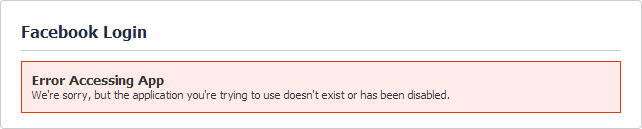
\includegraphics[width=0.5\textwidth]{figures/chapter4/ssoscan_study_FBError.png}
\caption{Facebook implementation error example}
\label{fig:ssoscan_study_FBError}
\end{figure}

\shortsection{Faulty implementations} To implement Facebook SSO, an application must be configured correctly in the Facebook developer center.  Using incorrect parameters to call the SSO entry point also result in errors that will prevent any user from authenticating to that application through SSO.  Such cases, automatically identified by SSOScan, were more common than we expected.  The most popular errors include setting the application to `sandbox' mode in the developer center for testing and development purposes (as shown in Figure~\ref{fig:ssoscan_study_FBError}), or providing a wrong application ID.  SSOScan found 39 (2.3\% out of 1660 sites that incorporate Facebook SSO buttons) sites that display visible Facebook SSO buttons but have implementations so buggy that no user could ever login using them.  A possible explanation is that the buttons are there for SEO purposes and the developers never actually bothered to implement it, or the developers simply copied and pasted an SSO snippet customized for another application without ever testing it.

\shortsection{Vulnerability trends} We found 205 sites (12.1\%) that misuse credentials (126 of which are misusing both access\_token and signed\_request) and 146 sites (8.6\%) that leak Facebook SSO credentials (of which 72 sites are leaking through both referrer headers and URLs).  A total of 345 sites (20.3\%) suffered from at least one vulnerability, and 3 sites suffered from both credential misuse and leakage problems.

As shown in Figure~\ref{fig:ssoscan_study_percentile} (b) and (c), the vulnerability rate does not appear to be strongly correlated with the site ranking.  Of the 1000 highest-ranked sites, 60 of the 270 (22.2\%) that support Facebook SSO are found to have at least one vulnerability.  The vulnerability rate is 21.3\% across all sites in the top 10,000 and 18.5\% for sites ranked from 10,001 to 20,000.  This indicates that development practices at larger companies do not appear to be more stringent (at least with respect to SSO) than they are at lower-profile sites.

\shortsection{Front-end Integration} There are three basic client-side methods to integrate Facebook SSO: a JavaScript SDK, a pre-configured widget, or a custom implementation.  (We have no way to determine how the developers are integrating Facebook SSO at the back end.)  We used SSOScan to aggregate front-end integration choices and compare them with vulnerability reports.  Table~\ref{tab:ssoscan_study_front-end} summarizes the results.  Websites using client side SDKs and pre-configured widgets are more likely to misuse credentials (29.1\% and 15.5\% vs. 1.3\% in non SDK/widget implementations).  Our guess is that this is due to the way SDKs and widgets conveniently expose raw \emph{access\_token}, \emph{signed\_request}, or even user name Facebook ID values.  This convenience may lead to the developers to neglect to check the signature and the intended audience of the credential.  However, our results also show that websites using SDKs and widgets are better in hiding credentials (3.6\% and 2.2\% compared to 12.4\% vulnerable rate in SDK/widget implementations).  This is likely because such applications use the Facebook-provided landing page which has safe redirect URLs and no third-party content.  Applications built this way are secure unless the developers explicitly add the credentials in the page content or URL.

\begin{table}[b]\centering
\begin{threeparttable}
\begin{tabular}{|c|r|r@{.}l|r@{.}l|}
\multicolumn{1}{c}{Method} & \multicolumn{1}{c}{Number} & \multicolumn{2}{c}{Misuse} & \multicolumn{2}{c}{Leakage} \\
\hline
SDK & 578 & 29 & 1\% & 3 & 6\%\\
\hline
Widget & 132 & 15 & 5\% & 2 & 2\%\\
\hline
Custom Code & 950 & 1 & 3\% & 12 & 4\%\\
\hline\hline
All & 1660  & 12 & 1\% & 8 & 6\%\\
\hline
\end{tabular}
\end{threeparttable}
\caption{Rate of credential misuse and credential leakage for different Facebook SSO front-end implementations}
\label{tab:ssoscan_study_front-end}
\end{table}

\shortsection{Vulnerable application examples} We list two examples of vulnerabilities found by SSOScan here to illustrate the potential risks.  Section~\ref{sec:ssoscan_deployment} discusses our experiences reporting them to site owners.

\shortsection{\url{ESPN.com}} ESPN, as shown in the example in Chapter~\ref{sec:ssoscan_manual_example}, is a sports and entertainment site that is the 16\textsuperscript{th}-ranked US website.  SSOScan found that \url{espn.com} is vulnerable to \emph{signed\_request} replacement attacks.  In addition to serving news content, \url{espn.com} also hosts fantasy sports leagues, including some played with real money at stake.  Damage caused by impersonation attacks can range from basic information stealing and comment posting to making changes to another player's fantasy teams.

\shortsection{\url{Match.com}} Ranked 118\textsuperscript{th} on the list, Match.com is a popular online dating website.  SSOScan revealed that \url{match.com} is also vulnerable to \emph{signed\_request} replacement attacks.  To use \url{match.com} services, users need to provide sensitive information including their birthday, location, photos, personal interests, and sexual orientation.  Impersonators will not only have access to this information, but also learn whom the victim is dating and possibly the time and location of the dates.

\shortsection{\url{Fodors.com}} Fordos is a travel advice website that is the 217\textsuperscript{th}-ranked US site.  Its redirection landing page contains \emph{access\_token} information along with some other third-party scripts in its content.  The scripts come from various sources including \url{quantserve.com}, \url{fonts.com}, \url{yahooapis.com}, and multiple domains owned by Google.  The permission Fordos requests includes user's basic information, email address, and more importantly, permission to post to user's wall on the his or her behalf. This means if the \emph{access\_token} is leaked to a malicious party, it can post to a user's Facebook wall without consent in addition to accessing the user's basic information. 


\subsection{Detection Accuracy}
\label{sec:toolEffectiveness}
To evaluate the detection accuracy of SSOScan, we sampled test cases from all results (including sites reported to have no Facebook SSO support, secure and vulnerable cases) and manually examined them.  We consider two types of mistakes --- misreporting whether the site integrates Facebook SSO, and misreporting whether a Facebook SSO-enabled website is vulnerable.  

\shortsection{Facebook Login Detection} SSOScan searches SSO button based on heuristics and cannot guarantee success for all websites. Indeed, it is not possible for anyone to determine with complete confidence if a website uses Facebook SSO by just browsing the site.  To roughly measure how many Facebook SSO-enabled websites were missed by SSOScan, we randomly sampled the 100 sites that were reported by SSOScan to have no Facebook SSO support and manually examined them.  To make the samples representative of the whole set, we picked one site out of every 200 sites ordered by their rank.  From manually investigating these 100 sites, we could only find one site that included Facebook SSO but was missed by SSOScan.  As we introduce later in Section~\ref{sec:ssoscan_deployment}, we also deployed SSOScan as a web service that is made available to use in our research group.  The web service has received a total of 69 valid submissions so far and we have also manually examined the vulnerability reports.\footnote{These have mostly been sites suggested by people we have demoed SSOScan scan to, since the service has not yet been publicized.  Hence, it is a small and non-representative sample, so not clear what we can conclude from this at this point.}  We found four cases (5.8\%) where a submitted site included Facebook SSO but SSOScan was not able to trigger it.

The sites that SSOScan fails to find Facebook login present unusual interfaces which our heuristics are not able to navigate to.  Specifically, \url{oovoo.com} and \url{bitdefender.com} do not show any login button on its homepage, but instead the user needs to click a `my account' button to initiate the login process.  The \url{sears.com} site displays a login button on its homepage, but the SSO process is not initiated until the user interacts with the pop-up window three times, which exceeds the maximum click depths (two) in this evaluation.  We have also seen one case (\url{coursesmart.com}) in which the login process is rather typical, but SSOScan still missed the correct login button (that button is scored the  4th highest while SSOScan only attempts to click the top 3 candidates.).  Most of these issues may be addressed with more relaxed restrictions and more regular expression matching as described in Section~\ref{sec:ssoscan_heuristics}.  Finally, our prototype implementation is limited to English-language websites due to its string matching algorithm, but could be extended to include keywords in other languages.

SSOScan may also incorrectly conclude that a website supports Facebook SSO when it does not.  We have seen sites (e.g., \url{msn.com}) that only use Facebook SSO to download user activities and display them on the page, but do not integrate their identity system with Facebook SSO.  Although SSOScan is designed to skip searching on typical Facebook-provided social plugins and widgets, non-standard integration of such functionalities may rarely lead to false positives.

\shortsection{Oracle Correctness} The Oracle determines if a user has logged in by searching the response for identifying information.  Information for the test account is chosen carefully to be unlikely to appear otherwise but to be close enough to real names to pass sanity checks.  For example, the randomly generated name ``Syxvq Ldswpk" was rejected by a small number of websites,  but ``Jiskamesda Quanarista" always passed sanity checks and only appeared in an authenticated session in all of our tests.

The Oracle checks the whole response for identifying information instead of only the DOM content to handle sites which only embed such information in first-party cookies after logging in.  In some rare cases, these cookies could be issued even before SSOScan finishes registration forms.  This means that before the Enroller searches for registration forms to fill in, the Oracle deems registration as unnecessary because it concludes that the application is already in an authenticated state.  Although SSOScan is able to proceed and determine vulnerability status, the application never enters an authenticated state and the report might be inaccurate.

\shortsection{Trusted Third-Party Domains} For credential leakage vulnerabilities, SSOScan reports an application as vulnerable if it identifies visible credentials co-existing with \emph{any} content or script that comes from \emph{any} origin other than the host or Facebook.  This could overestimate the vulnerable sites because the host may own other domains and serve content over them, which should not be considered untrusted.  For example, content delivery networks and sub-company scenarios (e.g. \url{cnn.com} embedding content from \url{turner.com}, but CNN is owned by Turner) are common among popular websites.

\subsection{Automation Failures}
\label{sec:ssoscan_study_automationFailReasons}

For about 19\% of the top 10,000 tested site that include functional Facebook SSO, SSOScan is not able to fully automate the checking process.  Figure~\ref{fig:ssoscan_study_errorStat} shows the distribution of rank of failed test websites.

\begin{figure}[hbt]
\centering
\includegraphics[width=0.7\textwidth]{figures/chapter4/ssoscan_study_errorStat}
\caption{Failed tests rank distribution}
\label{fig:ssoscan_study_errorStat}
\end{figure}

To better understand the reasons why SSOScan fails, we manually studied all 228 failed cases reported by SSOScan for sites ranked in the top 10,000.  We found that although 47 out of these 228 cases set their Facebook application configurations and SSO entry points properly, they never respond to credentials returned by Facebook SSO, which means no users would be able to successfully log into these sites through Facebook SSO.  Excluding these 47 left us a total of 181 failure cases.

\shortsection{Registration automation failure} By far, the most common reason for SSOScan to fail is due to complicated or highly-customized registration process.  We found 43.7\% of the sites that implement Facebook SSO still require users to perform additional actions to complete the registration (roughly evenly distributed by site popularity).  SSOScan failed to complete registration on 143 (33.6\%) of them.  Table~\ref{tab:ssoscan_study_failureReasons} shows the major reasons contributing to this failure ordered by their occurrences: 1) sites that require SSO users to link to an existing account or provide payment information to subscribe to the service; Currently SSOScan cannot handle the ``linking'' action: automatically registering a ``traditional'' account and perform the linking poses an out-of-scope challenge --- doing so often requires solving CAPTCHAs\footnote{On the contrary, most test applications (942 out of 973, see Section~\ref{sec:ssoscan_study_automationFailReasons}) do not ask users to solve CAPTCHAs when an account is created through SSO.  This is a reasonable practice, since the user who is able to provide a valid Facebook account should have already passed Facebook's Turing test, and adding additional CAPTCHAs would be unnecessarily annoying to the users.}; 2) registration forms that include CAPTCHAs; 3) special input elements (e.g. \code{div}, \code{span} or \code{image} as opposed to \code{input}) cannot be found automatically, or special requirements for the input that cannot be fulfilled; 4) sites where the registration submission button cannot be located; 5) sites that requires users to confirm email addresses before continuing (usually this involves clicking a link in an email sent by the server to the user's email address); and 6) sites that insecurely send registration data using a non-HTTPS form which causes the testing browser to pop up a warning and stall.


 \begin{table}[t]
 \begin{center}
 \begin{threeparttable}
 \begin{tabular}{|c|r|r@{.}l|}
 \hline
 \textbf{Failure reason} & \multicolumn{1}{|c|}{\textbf{Number}} & \multicolumn{2}{|c|}{\textbf{Percent}}\\
 \hline
 linking/subscription& 51 & 28 & 1\%\\
 \hline
 CAPTCHAs & 34 & 18 & 8\%\\
 \hline
 identity invisible to oracle & 28 & 15 & 5\%\\
 \hline
 atypical input elements & 20 & 11 & 0\%\\
 \hline
 atypical submit buttons & 19 & 10 & 5\%\\
 \hline
 email verification & 10 & 5 & 5\%\\
 \hline
 non-HTTPS submission forms & 9 & 5 & 0\%\\
 \hline
 other (e.g., timeouts) & 10 & 5 & 5\%\\
 \hline\hline
 Total failures & 181 & 100 &0\%\\
 \hline
 \end{tabular}
 \end{threeparttable}
 \end{center}
 \caption{Automation Failure Causes (top 10,000 sites)}
 \label{tab:ssoscan_study_failureReasons}
 \end{table}


\shortsection{Oracle confusion} SSOScan may also fail because the oracle reports failure (15.5\%), which occurs when it detects the login button no longer exists after Facebook SSO but cannot identify the session identity.  We manually analyzed such cases and found the biggest obstacle is that the application homepage does not include any identifying information at all.  For example, instead of showing `Welcome, \{username\}', it shows `Welcome, customer', or simply `Welcome', and the user name is only displayed when accessing the account information page.  In other cases, SSO authentication serves only a sub-service of the website such as its affiliated forum, but not the homepage which does not display any identifying information.

\shortsection{Others} During the testing, we have also seen a number of sites with extremely long loading time or inconsistent network latencies after Facebook SSO or upon navigating to certain pages.  While the latency spikes can likely be resolved by re-running the tests, frequent long delays which accumulate to SSOScan's maximum timeout will always halt the automation process.  For example, this happens when SSOScan accidentally triggers a browser confirmation dialog that requires user interaction, or asking users to stop a busy script execution.


\section{Heuristics Evaluation}
\label{sec:ssoscan_heuristics}

The ability of SSOScan to successfully complete the Facebook single sign-on and registration process depends on heuristics it uses to find buttons and fill in registration forms.  Since each attempted button click involves a high-latency round-trip with the server, early pruning of search space and prioritization of elements is important for achieving successful completion within a reasonable amount of time.

In this section, we explain in detail about some of the heuristics SSOScan use to quicken the search and improve the results.  We analyze the click data collected from the top 10,000 sites that use Facebook SSO (obtained from the large scale study) and show how tweaking the heuristics and significantly improve performance.

\subsection{SSOScan Options}
\label{sec:ssoscan_heuristics_options}

Each step in the automation process can be controlled by many options, including filters that can be enabled to eliminate candidate elements that are unlikely to be the correct target, weightings that adjust the contribution of different element properties to its score, and other behavior modifiers.  The ones SSOScan used when running the Section~\ref{sec:ssoscan_study} study are described below.

\begin{figure}[hbt]
\centering
\includegraphics[width=0.7\textwidth]{figures/chapter4/ssoscan_study_optionsExample}
\caption{Example corner cases}
\label{fig:ssoscan_study_optionsExample}
\end{figure}

\shortsection{Candidate rank} The button finder produces a candidate element list ranked by score.  SSOScan will first attempt clicking on the highest-ranked element, but sometimes the correct element is ranked lower.  This option controls how far down the list to attempt clicks until one is found that succeeds, or giving up.  For Section~\ref{sec:ssoscan_study}'s experiment, the lowest ranked element SSOScan clicks is the third.

\shortsection{Visibility filter} Most web sites only expect users to click on UI elements that are visible, so the button finder includes a filter that ignores all invisible elements (e.g., elements with zero height or width, shadowed in the background layer, or appear only when the user scrolls the initial screen position).  We describe how we implement this in Chapter~\ref{sec:ssoscan_heuristics_impl}.  %However, we found many cases where the user first hovers on an element which triggers a dropdown menu, and then the ``Login with Facebook'' button is displayed.  The visibility filter option selects whether invisible elements are considered as targets.

\shortsection{Position filter} We noticed that SSOScan sometimes gets distracted by a search box submit button when completing the registration form, even if it is able to correctly fill in the required information in all input elements.  To eliminate these misclicks, the position filter ignores submit buttons which are displayed above any inputs, based on our observation that the target registration form is always the bottom-most form on the landing page.

\shortsection{Registration form filter} As mentioned earlier in Section~\ref{sec:ssoscan_study_automationFailReasons}, many websites provide two actions for the user after SSO is completed: `create new account' or `link an existing account'.  The latter option requires the user to enter the user name and password of an existing account to finish the enrollment process.  To avoid these, the registration form filter ignores a candidate submit button if its parent form contains only two visible text inputs, one has the meaning of `name' or `email' and the other is of type password, since such an element is most likely to be a submit button of a linking form.

\shortsection{Element content matching} SSOScan searches for elements whose labels are close to ``login with Facebook'' for SSO buttons by default.  However, quite a few popular websites (e.g. \url{coupons.com}, right side of Figure~\ref{fig:ssoscan_study_optionsExample}) only allow users to ``sign up with Facebook'' first before logging in with Facebook.  If the user has yet to do this, attempting to login with Facebook will produce an error.  To handle this situation, SSOScan will search for elements with semantics similar to ``sign up with Facebook'' when it fails to register using the ``login'' buttons.

A filter may significantly reduce the number of mis\-clicks.  However, it may also occasionally exclude correct elements.  For example, not every correct submit button is below all inputs (e.g., left of Figure~\ref{fig:ssoscan_study_optionsExample}, and \url{expedia.com}'s submit button would have been missed with the element position filter enabled).  

Hence, SSOScan is designed to explore target sites using different option settings if enrollment does not succeed with the initial settings.  It will continue to attempt to complete the enrollment process using different settings until either the timeout threshold is reached or all configurations have been exhausted.  SSOScan also avoids doing duplicate work by detecting if a click attempt has resulted in a previously visited or completely explored state, which is described in more details in Chapter~\ref{sec:ssoscan_heuristics_impl}.

\subsection{Implementation}
\label{sec:ssoscan_heuristics_impl}

This chapter describes the techniques necessary to implement the previously mentioned filters.  

\shortsection{Determining element visibility} As introduced in Section~\ref{sec:ssoscan_heuristics_options}, SSOScan uses a filter that rejects elements which are not directly visible to the user.  We implement the filter by using \code{document.elementFromPoint} API.  For any given element \emph{E}, we first get its current top-left corner coordinates, width and length.  Then, \code{document.elementFromPoint} is called on ten points distributed equally along the diagonal inside this area.  If more than five of the elements returned are either \emph{E} itself or a child of \emph{E}, \emph{E} is considered to be on top.  Depending on current strategy, SSOScan may call \code{scrollIntoView} to include searching elements displayed at lower sections of a document.  Using \code{document.elementFromPoint}, however, has its limitations --- it always returns the underlying canvas element when called at any point on that canvas, therefore \code{onTopLayer} always returns false for elements placed on canvases.  We hope future browsers can fix this bug, but for now SSOScan relies on alternative option choices that does not ignore invisible buttons to handle such scenarios.

\shortsection{Avoiding futile and duplicate clicks} To further eliminate false positives in candidate lists as early as possible, SSOScan detects clicks which have no effect or have lead the web application into a previously visited state in the same attempt.  Na\"{\i}vely using URL or full \code{document.body.innerHTML} string to represent application state does not work well, because these information are not stable as variations exist across different requests and time (e.g. GET parameters and advertising content).  Fortunately, \code{getCandidates} provides a representative feature naturally --- the candidate list.  To detect previous clicks that are futile, SSOScan records candidate information before a click happens (line 17), and if any candidate list computed for subsequent clicks is exactly the same as previously recorded, SSOScan considers previous click(s) as futile and fast forward to the next candidate.  Similarly, SSOScan stores candidate information when the current state is fully explored, i.e. all candidates on the current page have been clicked or the number of attempts have reached a certain threshold, and if any future click lands on a page which matches the same set of candidates, SSOScan immediately moves on to the next candidate to avoid duplicate work.

To ensure SSOScan sees all candidate elements, we need to manually trigger event handlers upon selecting a particular option, and work around the same-origin policy to access elements in all \code{iframe}s.

\shortsection{Triggering Event Handlers} Programatically changing values of option, checkbox and radio elements using JavaScript does not trigger their \code{onChange} event handler.  However, in practice we have found several websites rely on this event handler to deliver different inputs to the user.  Therefore, we explicitly trigger the event handler after modifying element values.

\shortsection{Circumventing Same-Origin Policy} SSOScan needs to iterate through DOM elements while searching for candidates, but it cannot reach elements inside iframes from a different origin.  This is because the content scripts run as the principal of the host, and thus their accesses to iframes are subject to the same-origin policy.  However, we saw many cases where the target button is in an iframe which originates from the HTTPS domain of tested website.  To handle this, we inject content scripts into all iframes that have an HTTPS origin.  Excluding HTTP iframes will cause some content to be missed, however, including them generates problems as sites sometimes include iframes from a complete different website which may include SSO/submit buttons.  Besides, login and registration requests should be served over secure connections to prevent eavesdropping.  Some rare exceptions usually lead to more serious vulnerabilities such as password disclosure, but our prototype implementation does not check for this.

\subsection{Experiment Setup}
\label{sec:ssoscan_heuristics_heuristicsEval}

In theory, SSOScan could exhaustively trigger clicks on every element on the page (and on all response pages up to some maximum depth) which would result in nearly 100\% success rate.  This would be prohibitively slow in practice, though, so the number of attempted clicks must be limited for any realistic test.  Given the time needed for each click attempt, it is important to configure our scoring heuristics well to maximize the probability of a successful enrollment in the minimum amount of time.  

To gather statistics about the candidate elements, we modified SSOScan to try all possible strategies even if it has already \emph{found} the correct login button and to record information about all attempted clicks, including for example their size, position, visibility to the user, content string feature and whether it is \emph{successful}.  We define a click as \emph{successful} if it is included in any sequence of clicks from the start page to triggering the SSO process, regardless of whether it appeared in an attempt that failed to trigger the process.  Note that because SSOScan skips previously explored states to avoid redundant effort, it automatically rejects click sequences which involves cyclic state transitions, such as clicking on a random link and then clicking on a logo which leads the application back to its initial state.

We set up SSOScan to expand the candidate pool size for each configuration from 3 to 8, add more matching regular expressions (e.g., to match the string ``forum'' which occasionally leads to a login page on sites where no login is visible on the start page), and use equal weight for each of them.  We also removed all candidate filters described in Section~\ref{sec:ssoscan_heuristics_options}.  Our goal is to capture as many ways to trigger the SSO process as possible by doing as close to an exhaustive search as is feasible.  This increases the time required to scan a typical site to almost an hour (compared to a few minutes with the setup used in the full study), and does not include the registration or vulnerability status detection as it is only concerned with triggering the Facebook login process.

We ran the test on 973 sites from the top-10,000 ranked sites that were detected by SSOScan to support Facebook SSO in our main study (Section~\ref{sec:ssoscan_study}).  This biases the study slightly, since it only includes sites where the configuration used in the initial study is able to find Facebook SSO.  Ideally we would like to run all top-10,000 sites to avoid any bias introduced by the data set, but the significantly increased testing time prohibits us to do so, and the result of our subsequent study on a random sample of sites (Section~\ref{sec:ssoscan_heuristics_laterstudy}) supports that only few sites containing Facebook SSO were missed by the main study.

\subsection{Login Button Statistics}
\label{sec:ssoscan_heuristics_loginButtonStat}

The experiment recorded 29,539 unique\footnote{If two clicks happens on pages with the same URL, same element XPath and same element outerHTML, we consider them the same click.} click attempts, of which 5086 (17.2\%) are successful (that is, they either directly trigger SSO, or lead to subsequent clicks that trigger SSO).  This amounts to approximately 30 unique clicks attempted per site, but the number varies significantly based on the site design, from a few up to 109.

\begin{figure}[htb]
\centering
\includegraphics[width=0.8\textwidth]{figures/chapter4/ssoscan_heuristics_buttonType}
\caption{Login button type statistics}
\label{fig:ssoscan_heuristics_buttonType}
\end{figure}

\begin{figure}[htb]
\centering
\includegraphics[width=0.8\textwidth]{figures/chapter4/ssoscan_heuristics_buttonContent}
\caption{Login button content statistics}
\label{fig:ssoscan_heuristics_buttonContent}
\end{figure}

\shortsection{Element type and content} Figure~\ref{fig:ssoscan_heuristics_buttonType} shows how different button types and properties impact success rates.  We report the success rate as the number of times that element appeared as a successful click divided by the total number of clicks attempted on elements of that type.  The number beneath the element feature gives the total number of times that type of element occurred as a successful click target across all the test sites.  For example, the \emph{BUTTON} element type has an excellent success rate --- 60\% of all \emph{BUTTON} candidates are true positives for the Facebook SSO button.  But since it only appears as a successful click on 78 out of 973 sites in our sample, it is rarely useful.  By contrast, clicking on \emph{DIV} elements are much less likely to trigger the Facebook login, but such elements are more common.  The right side of Figure~\ref{fig:ssoscan_heuristics_buttonType} shows that elements that are directly visible to the user has a higher success rate than invisible ones, and elements residing in iframes are twice as likely to be the correct target as their counterparts in the main page.  These results suggest ways of weighting element types to improve the scoring function and increase the likelihood of finding successful clicks early.

Figure~\ref{fig:ssoscan_heuristics_buttonContent} shows how the success rate varies with attribute content (matched by the given regular expression).  The keyword ``oauth'' rarely exists in any content, but when it appears it is very likely to identify the target element.  The result also shows that ``FB'' is not a good indicator to predict the target, and we think this is probably because it is very short and may be used for similarly named JavaScript variables or random abbreviations.

Both figures include data for the \emph{first} click only (but do measure first click success based on subsequent clicks).  Data for the second clicks are noticeably different from the first, and overall success rates are lower on second clicks.  The most interesting fact we found is that ``connect'' (39\%) and ``Facebook'' (36\%) become the most successful matches of all regular expressions, followed by ``oauth'' at (26\%).  No other regular expressions exceed 20\% success for the second click.  

%This is likely because the second click always happen in a page
%or frame which contains many elements related to ``login'' (See bottom
%of Figure~\ref{fig:SSOButtonFinder}), and an element matching
%``Facebook'' would stand out as the correct candidate.  The figure also
%tells that the second click success rate is noticably lower than the
%first one, which is reasonable as a wrong first click could lead the
%application to a completely irrelevant page which SSOScan will then
%attempt multiple failure clicks.

\begin{figure}[htb]
\centering
\includegraphics[width=0.9\textwidth]{figures/chapter4/ssoscan_heuristics_widthHeight}
\caption{Impact of Login Button Size}
\label{fig:ssoscan_heuristics_widthHeight}
\end{figure}

\shortsection{Element size} Figure~\ref{fig:ssoscan_heuristics_widthHeight} gives the cumulative distribution function of the width and height of target elements.  For example, the 80\textsuperscript{th} percentile width of the true positive elements is approximately 150px, compared to 300px for false positive elements.  We did not find any significant difference between first and second clicks, so the figure combines data from all clicks.  The key result is that wide elements are less likely to be true positives, possibly due to SSOScan incorrectly including many large underlay elements as candidates.  The result is similar for element height (the lower two lines in the figure).  This suggests that it would be useful to add a filter function that excludes candidates whose width is greater than 300px.  We would expect it to eliminate 20\% of the false positives while hardly missing any of the true positives.  Alternatively, SSOScan could adjust the final score of a node according to its size based on these results.

\begin{figure}[tb]
\centering
\includegraphics[width=0.9\textwidth]{figures/chapter4/ssoscan_heuristics_density}
\caption{Login button location heatmap}
\label{fig:ssoscan_heuristics_density}
\end{figure}

\shortsection{Element position} Figure~\ref{fig:ssoscan_heuristics_density} shows the heatmap of the login button's position in a page.  The intensity at a location indicates the number of elements found there satisfying the property.  Only visible elements are shown, and each successful click only attributes to the intensity once.  All four figures are normalized with respect to their maximum intensity (i.e., element density).

The figures show an interesting distinction from first click to second click: successful first clicks almost exclusively appear in the upper right corner of the page, while the second click appears generally in the upper-middle part of a page.  The false positives are relatively more scattered everywhere on the page\footnote{The figures also show a clear width boundary.  In the experiments the browser resolution is 1920x1200, and it seems that most developers' designs follow a standard width of approximately 960px, which is why the density appears to be cut off.}.  This result suggest we should assign a higher weight for elements for these locations, and focus on elements in the vicinity of the upper right corner for the first click.  We could potentially even ignore the other criteria and only consider position to find login buttons on foreign-language sites.

Another potential improvement that we can learn from this result is the better sequence to retry different strategies.  Assuming a strategy places restrictions on candidates that they must be visible and smaller than 300px.  We learned from Figure~\ref{fig:ssoscan_heuristics_buttonType} and Figure~\ref{fig:ssoscan_heuristics_widthHeight} that successful clicks on invisible elements are far more common than elements larger than 300px.  Therefore, if this particular strategy fails to find the correct element, the immediate next strategy to try should expand search to invisible elements, but rather than larger ones.

\subsection{Validation}
\label{sec:ssoscan_heuristics_laterstudy}

After incorporating what we learned from these results (e.g., weight adjustment for different button sizes and types), we reran the SSOScan with the new heuristics on the sites ranked from 10,000 to 20,000 that SSOScan determined to support Facebook in the original study, which were not included in the heuristics evaluation.  We compare the results with those obtained by using a ``control'' version of SSOScan, with equal weights on all features and no candidate filtering.  All other settings such as candidate pool size are the same between two versions.

The results support the hypothesis that adjusting heu\-ri\-stics according to the results of the evaluation can improve the speed and robustness of detection of Facebook SSO integrations.  The na\"{\i}ve control version missed 72 out of the 601 sites while the new heuristics missed only two.  The average rank of correct candidate elements for the first and second click is 1.32 and 1.23 for the control experiment, which improves to 1.23 and 1.17 respectively with the new heuristics.

We also randomly picked 500 random sites from the sites that SSOScan have yet to find Facebook support in the experiment in Chapter~\ref{sec:ssoscan_study}.  We tested the expanded heuristics on these sites, and further increased the maximum click depth to three to see if more SSO integrations could be found.  Individual tests took an average of 31 minutes to finish, but varies significantly from a few minutes up to an hour (threshold) based on site content.

Four additional sites were found that support Facebook SSO from this sample in total.  Two are found due to the added regular expression \code{[Ff][Oo][Rr][Uu][Mm]}, one of which required 3 clicks to trigger the SSO process.  Another site is found due to the improved candidate ranking algorithm, and the fourth was found using the new candidate selection method that includes all elements in the right corner of the page, even if they do not match any regular expressions.  This provides a reasonable degree of confidence that our original study found a large enough fraction of all the popular sites using Facebook SSO to be representative, although likely missed around 1\% of Facebook SSO sites.  We did not try click depths greater than 3 because of the exponential time growth required to complete each test, but we feel confident that the number of Facebook SSO interfaces that can only be discovered by attempting more than 3 clicks is very low.

\section{Vendor Response and Deployment}
\label{sec:ssoscan_deployment}

In this chapter, we share our experiences reporting vulnerabilities, and suggesting ways SSOScan can be deployed to help secure applications integrating SSO services.

\subsection{Developer Responses}
\label{sec:ssoscan_deployment_developerResponses}

We started contacting the site owners soon after obtaining our first list of vulnerable sites, sending out notifications to 20 vulnerable websites that we thought were interesting.  We contacted them either through email or by submitting forms on their website.  The responses were very disappointing, compared with previous experiences reporting SDK-level vulnerabilities to identity providers in Chapter~\ref{sec:explication}.  The vulnerabilities found by SSOScan, on the other hand, are primarily in consumer-oriented sites without dedicated security teams or clear ways to effectively report security issues.  Of the 20 notifications, we only received 8 responses, most of which appear to be automated.  After the initial response, three websites sent us follow-up status updates.  \url{Espn.com} thanked us and told us the message has been passed onto appropriate personnel, but no follow up actions ensued.  One of \url{answers.com}'s engineers asked us for more details, but failed to respond again after we replied with proposed fix.  As of the time writing, both sites are still vulnerable.  Four months after getting the automated reply from \url{ehow.com}, we received a response stating that they have removed Facebook SSO from their website due to ``content deemed inappropriate'', and we have confirmed that the Facebook SSO button has indeed been removed.  Sadly, we think their staff likely did not (bother to) understand our explanation for the fix and simply removed the feature for their convenience.

The other instance where a reported vulnerability was fixed was for \url{hipmunk.com}.  Hipmunk was found to be vulnerable to both the \emph{access\_token} and \emph{signed\_request} replacement attacks.  We did not get any response from Hipmunk when the vulnerability was reported through the normal channels, but through a personal connection we were able to contact them directly.  This led to a quick response and series of emails with one of Hipmunk's engineers.  We explained how to check the signature of a \emph{signed\_request}, which should fix both vulnerabilities.  However, when they got back to us believing that the fix was complete, we re-ran SSOScan and found that Hipmunk was still vulnerable to the \emph{access\_token} replacement attack.  This meant Hipmunk checked the signature of \emph{signed\_request} after the fix, but never decoded the signed message body and compared its Facebook ID with the one returned by exchanging \emph{access\_token}.  This surprised us, as we implicitly assumed the developers will consume the signed message body after verifying its signature, and thus only included `verifying signature' in the proposed fix.  After further explanation, the site was fixed and now passes all our tests.

\subsection{Deployment}\label{sec:deployment}
Our experiences reporting vulnerabilities found by SSOScan suggest that notifying vendors individually will have little impact, which is consistent with experiences reported by Wang et al. with online stores~\cite{Wang:2011:SFO:2006077.2006782}.  Hence, we consider two alternate ways of deploying SSOScan to improve the security of integrated applications.

\shortsection{App center integration} We believe SSOScan would be most effective when used by an application distribution center (e.g. Apple store, Google Play) or identity provider (e.g., Facebook) as part of the application validation process.  The identity provider has a strong motivation to protect users who use its service for SSO, and could use SSOScan to identify sites that can compromise those users.  It could then deliver warning messages to visitors of vulnerable applications during the log in through Facebook SSO process, or even go so far as to shut down SSO logins for that application.  We also believe our results can provide guidance to vendors developing SSO services.  The results in Chapter~\ref{sec:ssoscan_study_generalstats} indicate that sites are more likely to misuse credentials when using the Facebook JavaScript SDK.  With Facebook's help, this problem could be mitigated by placing detailed instructions inside the SDK.  The instructions could be presented as (non-executable) code in the SDK rather than as comments, so that the developers cannot get by without reading and removing them.

\shortsection{Checking-as-a-service} Without involving an centralized infrastructure, the best opportunity to deploy SSOScan is as a vulnerability scanning service that developers can use to check their implementations before their applications are launched (our prototype service at \url{http://www.ssoscan.org/} can be used for this now).  For a developer-directed test, it would be reasonable to ask the developer to either guide the tool through the registration process or provide a special test account that bypasses this step in cases where it cannot be fully automated.  Even if we assume no aid from the developers, they should at least be able to tolerate a longer testing time than is feasible in doing a large-scale scan.